\setmodule{7}

%BEGIN_FOLD % ====>>_____ Занятие 1 _____<<====
\begin{class}[number=1]
	\begin{listofex}
		\item Два ребра прямоугольного параллелепипеда, выходящие из одной вершины, равны \(1, 2\). Объем параллелепипеда равен \(6\). Найдите площадь его поверхности.
		\item Два ребра прямоугольного параллелепипеда равны \(7\) и \(4\), а объём параллелепипеда равен \(140\). Найдите площадь поверхности этого параллелепипеда.
		\item 
		\begin{minipage}[t]{\bodywidth}
			В прямоугольном параллелепипеде \(ABCDA_1B_1C_1D_1\) рёбра \(AB, BC\) и диагональ боковой грани \(BC_1\) равны соответственно \(7, \) \( 3\) и \(3\sqrt{5}\). Найдите объём параллелепипеда \(ABCDA_1B_1C_1D_1\).
		\end{minipage}
		\hspace{0.02\linewidth}
		\begin{minipage}[t]{\picwidth}
			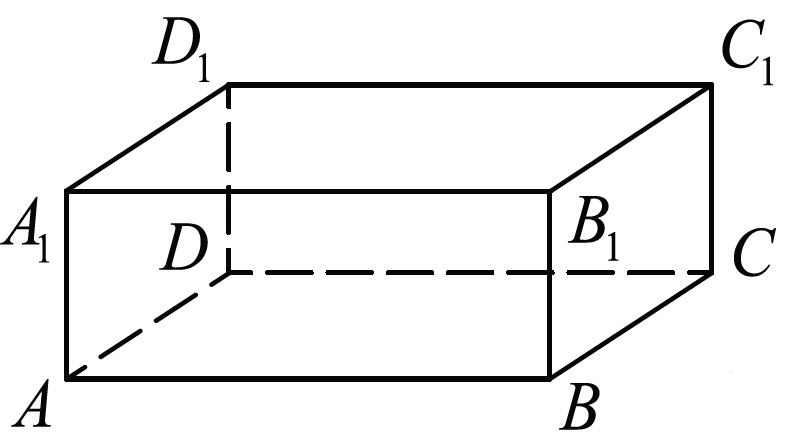
\includegraphics[align=t, width=\linewidth]{\picpath/G101M9L1-1}
		\end{minipage}
		\item 
		\begin{minipage}[t]{\bodywidth}
			В прямоугольном параллелепипеде \(ABCDA_1B_1C_1D_1\) рёбра \(CD, CB\) и диагональ \(CD_1\) боковой грани равны соответственно \(2, 4\) и \(2\sqrt{10}\). Найдите площадь поверхности параллелепипеда \(ABCDA_1B_1C_1D_1\).
		\end{minipage}
		\hspace{0.02\linewidth}
		\begin{minipage}[t]{\picwidth}
			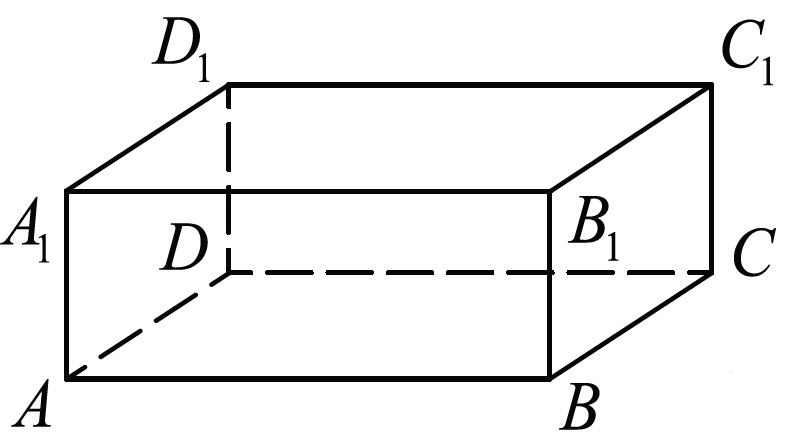
\includegraphics[align=t, width=\linewidth]{\picpath/G101M9L1-1}
		\end{minipage}
		\item Основанием прямой треугольной призмы служит прямоугольный треугольник с катетами \(6\) и \(8\), боковое ребро равно \(5\). Найдите объем призмы.
		\item В основании прямой призмы лежит прямоугольный треугольник, один из катетов которого равен \(2\), а гипотенуза равна \(\sqrt{53}\). Найдите объём призмы, если её высота равна \(3\).
		\item В основании прямой призмы лежит прямоугольный треугольник, катеты которого равны \(11\) и \(5\). Найдите объём призмы, если её высота равна \(4\).
		\item 
		\begin{minipage}[t]{\bodywidth}
			Стороны основания правильной шестиугольной пирамиды равны \(10\), боковые ребра равны \(13\). Найдите площадь боковой поверхности этой пирамиды.
		\end{minipage}
		\hspace{0.02\linewidth}
		\begin{minipage}[t]{\picwidth}
			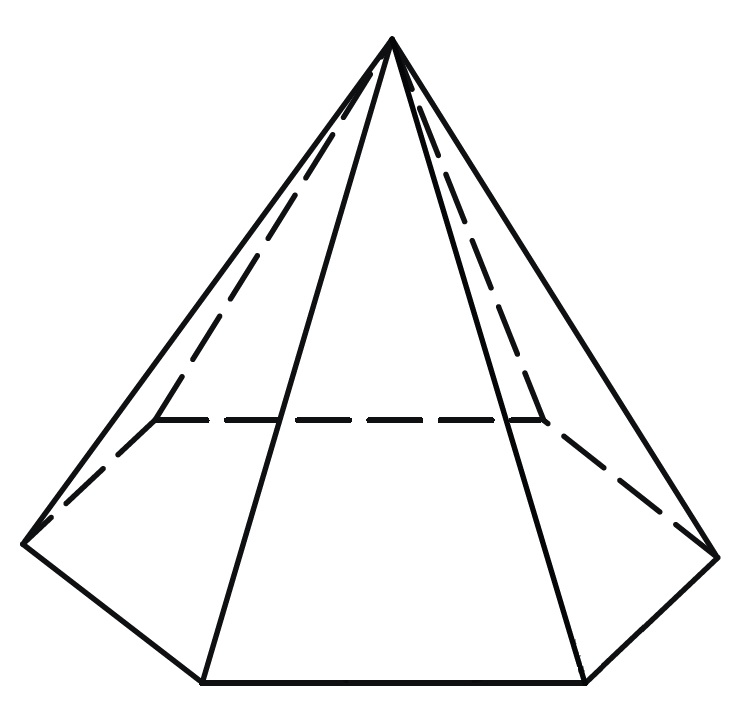
\includegraphics[align=t, width=\linewidth]{\picpath/G101M9L1-2}
		\end{minipage}
		\item 
		\begin{minipage}[t]{\bodywidth}
			Основанием пирамиды является прямоугольник со сторонами \(3\) и \(4\). Ее объем равен \(16\). Найдите высоту этой пирамиды.
		\end{minipage}
		\hspace{0.02\linewidth}
		\begin{minipage}[t]{\picwidth}
			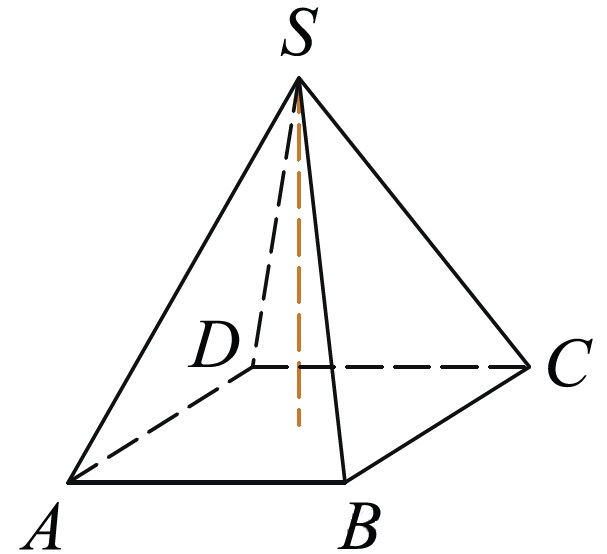
\includegraphics[align=t, width=\linewidth]{\picpath/G101M9L1-3}
		\end{minipage}
		\item 
		\begin{minipage}[t]{\bodywidth}
			Основанием пирамиды является прямоугольник со сторонами \(4\) и \(5\). Ее объем равен \(80\). Найдите высоту этой пирамиды.
		\end{minipage}
		\hspace{0.02\linewidth}
		\begin{minipage}[t]{\picwidth}
			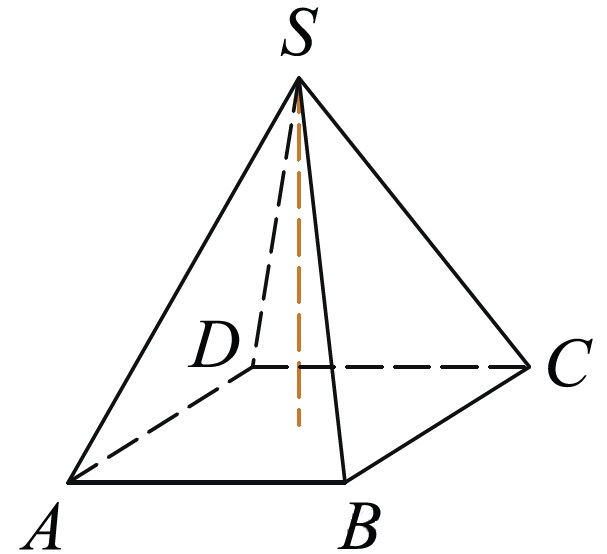
\includegraphics[align=t, width=\linewidth]{\picpath/G101M9L1-3}
		\end{minipage}
		\item 
		\begin{minipage}[t]{\bodywidth}
			Найдите объём правильной четырёхугольной пирамиды, сторона основания которой равна \(4\), а боковое ребро равно \(\sqrt{17}\).
		\end{minipage}
		\hspace{0.02\linewidth}
		\begin{minipage}[t]{\picwidth}
			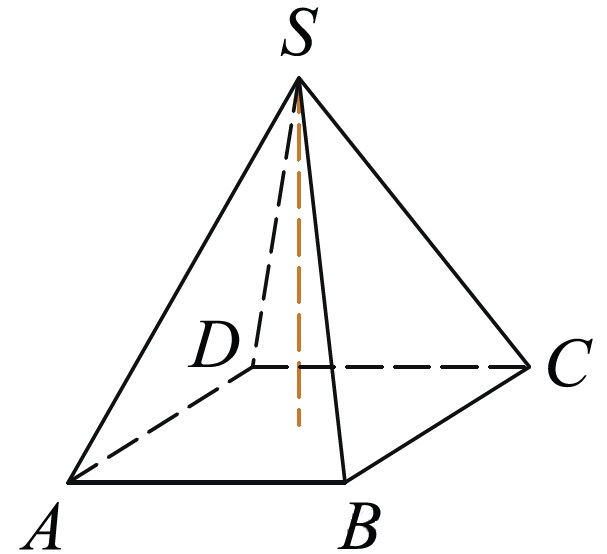
\includegraphics[align=t, width=\linewidth]{\picpath/G101M9L1-3}
		\end{minipage}
		\item 
		\begin{minipage}[t]{\bodywidth}
			В основании пирамиды \(SABC\) лежит правильный треугольник \(ABC\) со стороной \(10\), а боковое ребро \(SA\) перпендикулярно основанию и равно Найдите объём пирамиды \(SABC\).
		\end{minipage}
		\hspace{0.02\linewidth}
		\begin{minipage}[t]{\picwidth}
			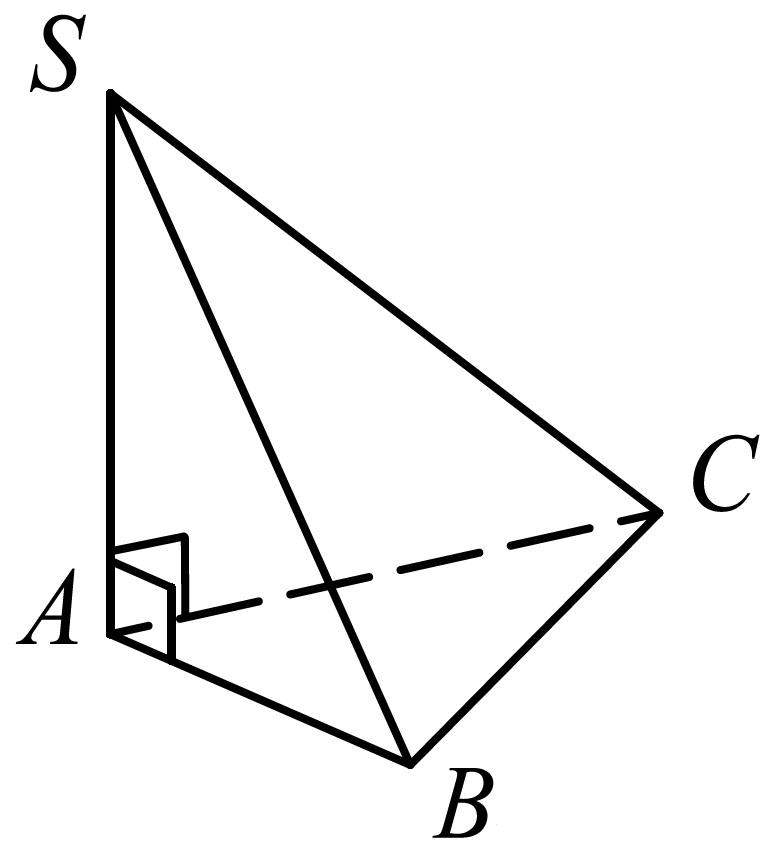
\includegraphics[align=t, width=\linewidth]{\picpath/G101M9L1-4}
		\end{minipage}
		\item 
		\begin{minipage}[t]{\bodywidth}
			В треугольной пирамиде \(ABCD\) рёбра \(AB, AC\) и \(AD\) взаимно перпендикулярны. Найдите объём этой пирамиды, если \(AB = 6, AC = 18\) и \(AD = 8\).
		\end{minipage}
		\hspace{0.02\linewidth}
		\begin{minipage}[t]{\picwidth}
			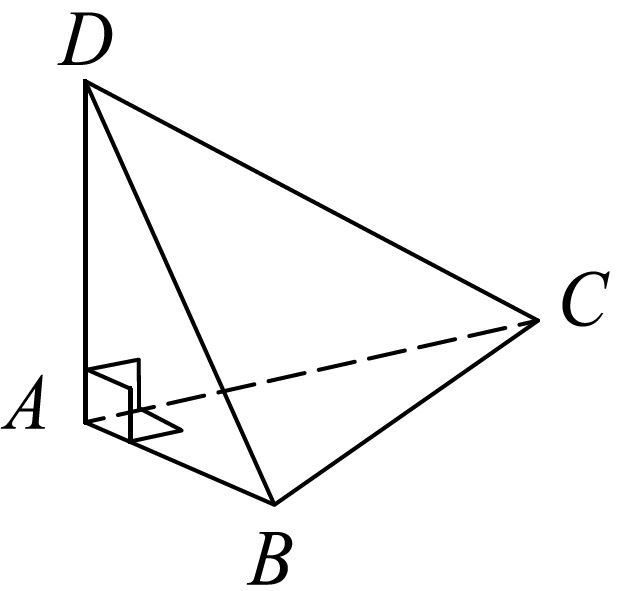
\includegraphics[align=t, width=\linewidth]{\picpath/G101M9L1-5}
		\end{minipage}
		\newpage
		\item Стороны основания правильной треугольной пирамиды равны \(16\), а боковые рёбра равны \(10\). Найдите площадь боковой поверхности пирамиды.
		\item Даны два цилиндра. Радиус основания и высота первого равны соответственно \(4\) и \(18\), а второго --- \(2\) и \(3\). Во сколько раз площадь боковой поверхности первого цилиндра больше площади боковой поверхности второго?
		
		
		%\item 
		%\begin{minipage}[t]{\bodywidth}
		%	
		%\end{minipage}
		%\hspace{0.02\linewidth}
		%\begin{minipage}[t]{\picwidth}
		%	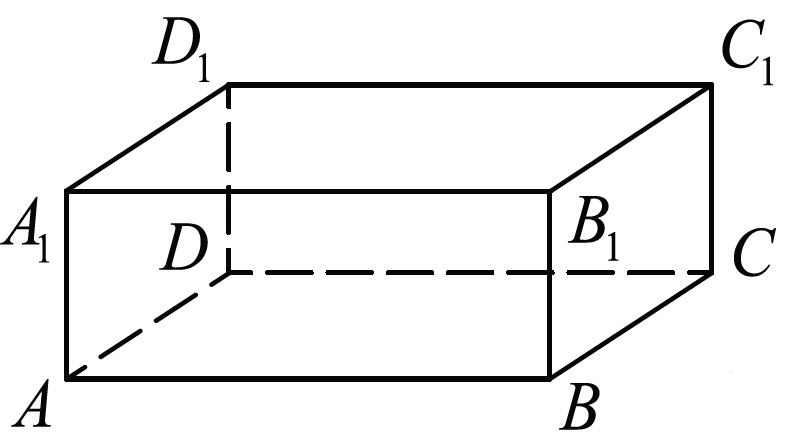
\includegraphics[align=t, width=\linewidth]{\picpath/G101M9L1-1}
		%\end{minipage}
	\end{listofex}
\end{class}
%END_FOLD

%BEGIN_FOLD % ====>>_____ Занятие 2 _____<<====
\begin{class}[number=2]
	\begin{listofex}
		\item Занятие 2
	\end{listofex}
\end{class}
%END_FOLD

%BEGIN_FOLD % ====>>_ Домашняя работа 1 _<<====
\begin{homework}[number=1]
	\begin{listofex}
		
		\item Основанием прямой треугольной призмы служит прямоугольный треугольник с катетами \(12\) и \(5\), боковое ребро равно \(6\). Найдите объем призмы.
		\item В основании прямой призмы лежит прямоугольный треугольник, катеты которого равны по \(12\). Найдите объём призмы, если её высота равна \(2\).
		\item Два ребра прямоугольного параллелепипеда, выходящие из одной вершины, равны \(4, 6\). Объем параллелепипеда равен \(48\). Найдите площадь его поверхности.
		\item 
		\begin{minipage}[t]{\bodywidth}
			В основании пирамиды \(SABC\) лежит правильный треугольник \(ABC\) со стороной \(4\), а боковое ребро \(SA\) перпендикулярно основанию и равно \(7\) Найдите объём пирамиды \(SABC\).
		\end{minipage}
		\hspace{0.02\linewidth}
		\begin{minipage}[t]{\picwidth}
			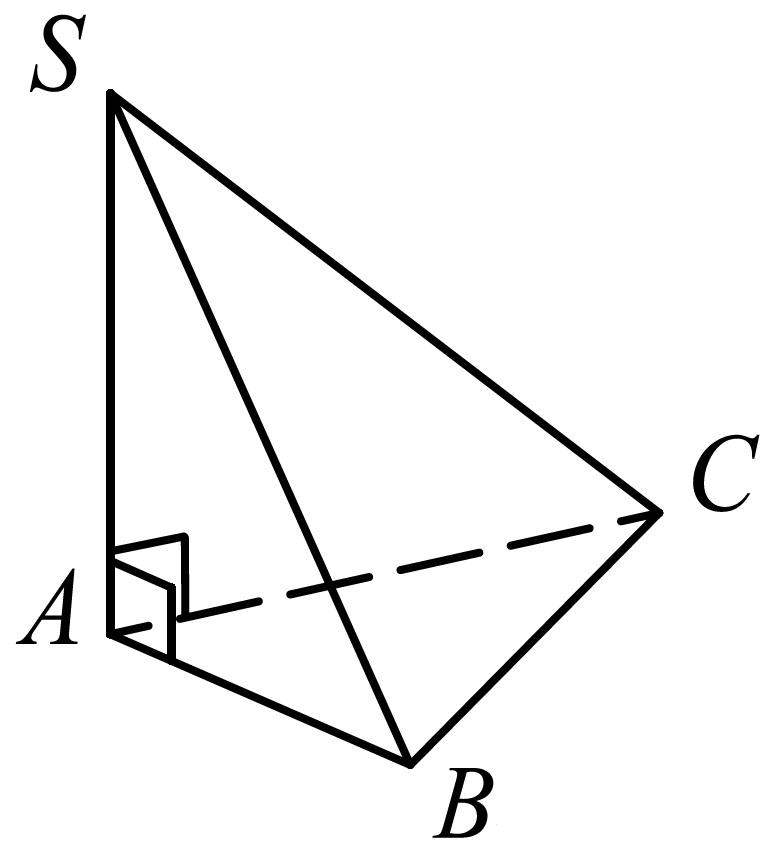
\includegraphics[align=t, width=\linewidth]{\picpath/G101M9L1-4}
		\end{minipage}
		\item Объём конуса равен \(50\pi \), а его высота равна \(6\). Найдите радиус основания конуса.
		\item Даны два конуса. Радиус основания и образующая первого конуса равны, соответственно, \(2\) и \(4\), а второго --- \(6\) и \(8\). Во сколько раз площадь боковой поверхности второго конуса больше площади боковой поверхности первого?
		\item Даны два конуса. Радиус основания и высота первого конуса равны соответственно \(9\) и \(2\), а второго --- \(3\) и \(3\). Во сколько раз объём первого конуса больше объёма второго?
		\item Даны два шара с радиусами \(5\) и \(1\). Во сколько раз площадь поверхности первого шара больше площади поверхности второго?
		\item Даны два шара с радиусами \(4\) и \(1\). Во сколько раз объём большего шара больше объёма другого?
		\item Даны два шара с радиусами \(9\) и \(3\). Во сколько раз площадь поверхности большего шара больше площади поверхности меньшего?
	\end{listofex}
\end{homework}
%END_FOLD

%BEGIN_FOLD % ====>>_____ Занятие 3 _____<<====
\begin{class}[number=3]
	\begin{listofex}
		\item Стороны основания правильной треугольной пирамиды равны \(16\), а боковые рёбра равны \(10\). Найдите площадь боковой поверхности пирамиды.
		\item Даны два цилиндра. Радиус основания и высота первого равны соответственно \(4\) и \(18\), а второго --- \(2\) и \(3\). Во сколько раз площадь боковой поверхности первого цилиндра больше площади боковой поверхности второго?
		\item Объём конуса равен \(108\pi \), а его высота равна \(3\). Найдите радиус основания конуса.
		\item Даны два конуса. Радиус основания и образующая первого конуса равны, соответственно, \(5\) и \(4\), а второго --- \(10\) и \(8\). Во сколько раз площадь боковой поверхности второго конуса больше площади боковой поверхности первого?
		\item Даны два конуса. Радиус основания и высота первого конуса равны соответственно \(5\) и \(10\), а второго --- \(3\) и \(2\). Во сколько раз объём первого конуса больше объёма второго?
		\item Даны два шара с радиусами \(8\) и \(11\). Во сколько раз площадь поверхности первого шара больше площади поверхности второго?
		\item Даны два шара с радиусами \(2\) и \(8\). Во сколько раз объём большего шара больше объёма другого?
		\item Даны два шара с радиусами \(6\) и \(14\). Во сколько раз площадь поверхности большего шара больше площади поверхности меньшего?
		\item Теплоход проходит по течению реки до пункта назначения \(255\) км и после стоянки возвращается в пункт отправления. Найдите скорость теплохода в неподвижной воде, если скорость течения равна \(1\) км/ч, стоянка длится \(2\) часа, а в пункт отправления теплоход возвращается через \(34\) часа после отплытия из него. Ответ дайте в км/ч.
		\item Моторная лодка в \(10:00\) вышла из пункта \(A\) в пункт \(B\), расположенный в \(30\) км от \(A\). Пробыв в пункте \(B\) \(2\) часа \(30\) минут, лодка отправилась назад и вернулась в пункт \(A\) в \(18:00\). Определите (в км/ч) собственную скорость лодки, если известно, что скорость течения реки \(1\) км/ч.
		\item Теплоход, скорость которого в неподвижной воде равна \(25\) км/ч, проходит по течению реки и после стоянки возвращается в исходный пункт. Скорость течения равна \(3\) км/ч, стоянка длится \(5\) часов, а в исходный пункт теплоход возвращается через \(30\) часов после отплытия из него. Сколько километров прошел теплоход за весь рейс?
		\item Теплоход проходит по течению реки до пункта назначения \(200\) км и после стоянки возвращается в пункт отправления. Найдите скорость течения, если скорость теплохода в неподвижной воде равна \(15\) км/ч, стоянка длится \(10\) часов, а в пункт отправления теплоход возвращается через \(40\) часов после отплытия из него. Ответ дайте в км/ч.
		\item Пристани \(A\) и \(B\) расположены на озере, расстояние между ними \(390\) км. Баржа отправилась с постоянной скоростью из \(A\) в \(B\). На следующий день после прибытия она отправилась обратно со скоростью на \(3\) км/ч больше прежней, сделав по пути остановку на \(9\) часов. В результате она затратила на обратный путь столько же времени, сколько на путь из \(A\) в \(B\). Найдите скорость баржи на пути из \(A\) в \(B\). Ответ дайте в км/ч.
		\item Моторная лодка прошла против течения реки \(112\) км и вернулась в пункт отправления, затратив на обратный путь на \(6\) часов меньше. Найдите скорость течения, если скорость лодки в неподвижной воде равна \(11\) км/ч. Ответ дайте в км/ч.
	\end{listofex}
\end{class}
%END_FOLD

%BEGIN_FOLD % ====>>_____ Занятие 4 _____<<====
\begin{class}[number=4]
	\begin{listofex}
		\item Найдите корень уравнения: \( 2^{2x-3}=2^{2x-2} \).
		\item Найдите корень уравнения: \( 2^{4-2x}=64 \).
		\item Найдите корень уравнения: \( 5^{x-7}=\dfrac{ 1 }{ 125 } \).
		\item Найдите корень уравнения: \( \left( \dfrac{ 1 }{ 3 } \right)^{x-8}=\dfrac{ 1 }{ 9 } \).
		\item Найдите корень уравнения: \( \left( \dfrac{ 1 }{ 2 } \right)^{6-2x}=4 \).
		\item Найдите корень уравнения: \( 16^{x-9}=0,5 \).
		\item Найдите корень уравнения: \( \left( \dfrac{ 1 }{ 9 } \right)^{x-13}=3 \).
		\item Найдите корень уравнения: \( 9^{-5+x}=729 \).
		
		
		
		
		\item Пристани \(A\) и \(B\) расположены на озере, расстояние между ними \(390\) км. Баржа отправилась с постоянной скоростью из \(A\) в \(B\). На следующий день после прибытия она отправилась обратно со скоростью на \(3\) км/ч больше прежней, сделав по пути остановку на \(9\) часов. В результате она затратила на обратный путь столько же времени, сколько на путь из \(A\) в \(B\). Найдите скорость баржи на пути из \(A\) в \(B\). Ответ дайте в км/ч.
		\item Моторная лодка прошла против течения реки \(112\) км и вернулась в пункт отправления, затратив на обратный путь на \(6\) часов меньше. Найдите скорость течения, если скорость лодки в неподвижной воде равна \(11\) км/ч. Ответ дайте в км/ч.
		
		\item На изготовление \(475\) деталей первый рабочий тратит на \(6\) часов меньше, чем второй рабочий на изготовление \(550\) таких же деталей. Известно, что первый рабочий за час делает на \(3\) детали больше, чем второй. Сколько деталей в час делает первый рабочий?
		\item Первая труба пропускает на \(3\) литра воды в минуту меньше, чем вторая. Сколько литров воды в минуту пропускает первая труба, если резервуар объемом \(108\) литров она заполняет на \(3\) минуты дольше, чем вторая труба?
		\item Первый насос наполняет бак за \(20\) минут, второй --- за \(30\) минут, а третий --- за \(1\) час. За сколько минут наполнят бак три насоса, работая одновременно?
		\item Игорь и Паша красят забор за \(9\) часов. Паша и Володя красят этот же забор за \(12\) часов, а Володя и Игорь --- за \(18\) часов. За сколько часов мальчики покрасят забор, работая втроем?
		\item Заказ на \(156\) деталей первый рабочий выполняет на \(1\) час быстрее, чем второй. Сколько деталей за час изготавливает первый рабочий, если известно, что он за час изготавливает на \(1\) деталь больше второго?
		\item Первый и второй насосы наполняют бассейн за \(9\) минут, второй и третий --- за \(14\) минут, а первый и третий --- за \(18\) минут. За сколько минут эти три насоса заполнят бассейн, работая вместе?
		
		
		
		%\item Первая труба пропускает на \(8\) литров воды в минуту меньше, чем вторая. Сколько литров воды в минуту пропускает первая труба, если резервуар объемом \(660\) литров она заполняет на \(11\) минут дольше, чем вторая труба заполняет резервуар объемом \(570\) литров?
	\end{listofex}
\end{class}
%END_FOLD

%BEGIN_FOLD % ====>>_ Домашняя работа 2 _<<====
\begin{homework}[number=2]
	\begin{listofex}
		\item Домашняя работа 2
	\end{listofex}
\end{homework}
%END_FOLD

%BEGIN_FOLD % ====>>_____ Занятие 5 _____<<====
\begin{class}[number=5]
	\begin{listofex}
		\item Занятие 5
	\end{listofex}
\end{class}
%END_FOLD

%BEGIN_FOLD % ====>>_____ Занятие 6 _____<<====
\begin{class}[number=6]
	\begin{listofex}
		\item Занятие 6
	\end{listofex}
\end{class}
%END_FOLD

%BEGIN_FOLD % ====>>_ Домашняя работа 3 _<<====
\begin{homework}[number=3]
	\begin{listofex}
		\item Домашняя работа 3
	\end{listofex}
\end{homework}
%END_FOLD

%BEGIN_FOLD % ====>>_____ Занятие 7 _____<<====
\begin{class}[number=7]
	\title{Подготовка к проверочной}
	\begin{listofex}
		\item Занятие 7
	\end{listofex}
\end{class}
%END_FOLD

%BEGIN_FOLD % ====>>_ Проверочная работа _<<====
\begin{exam}
	\begin{listofex}
		\item Проверочная
	\end{listofex}
\end{exam}
%END_FOLD